
\subsection{package edu.kit.pse.fridget.client.service}
\begin{figure}[H]
	       \centering
	       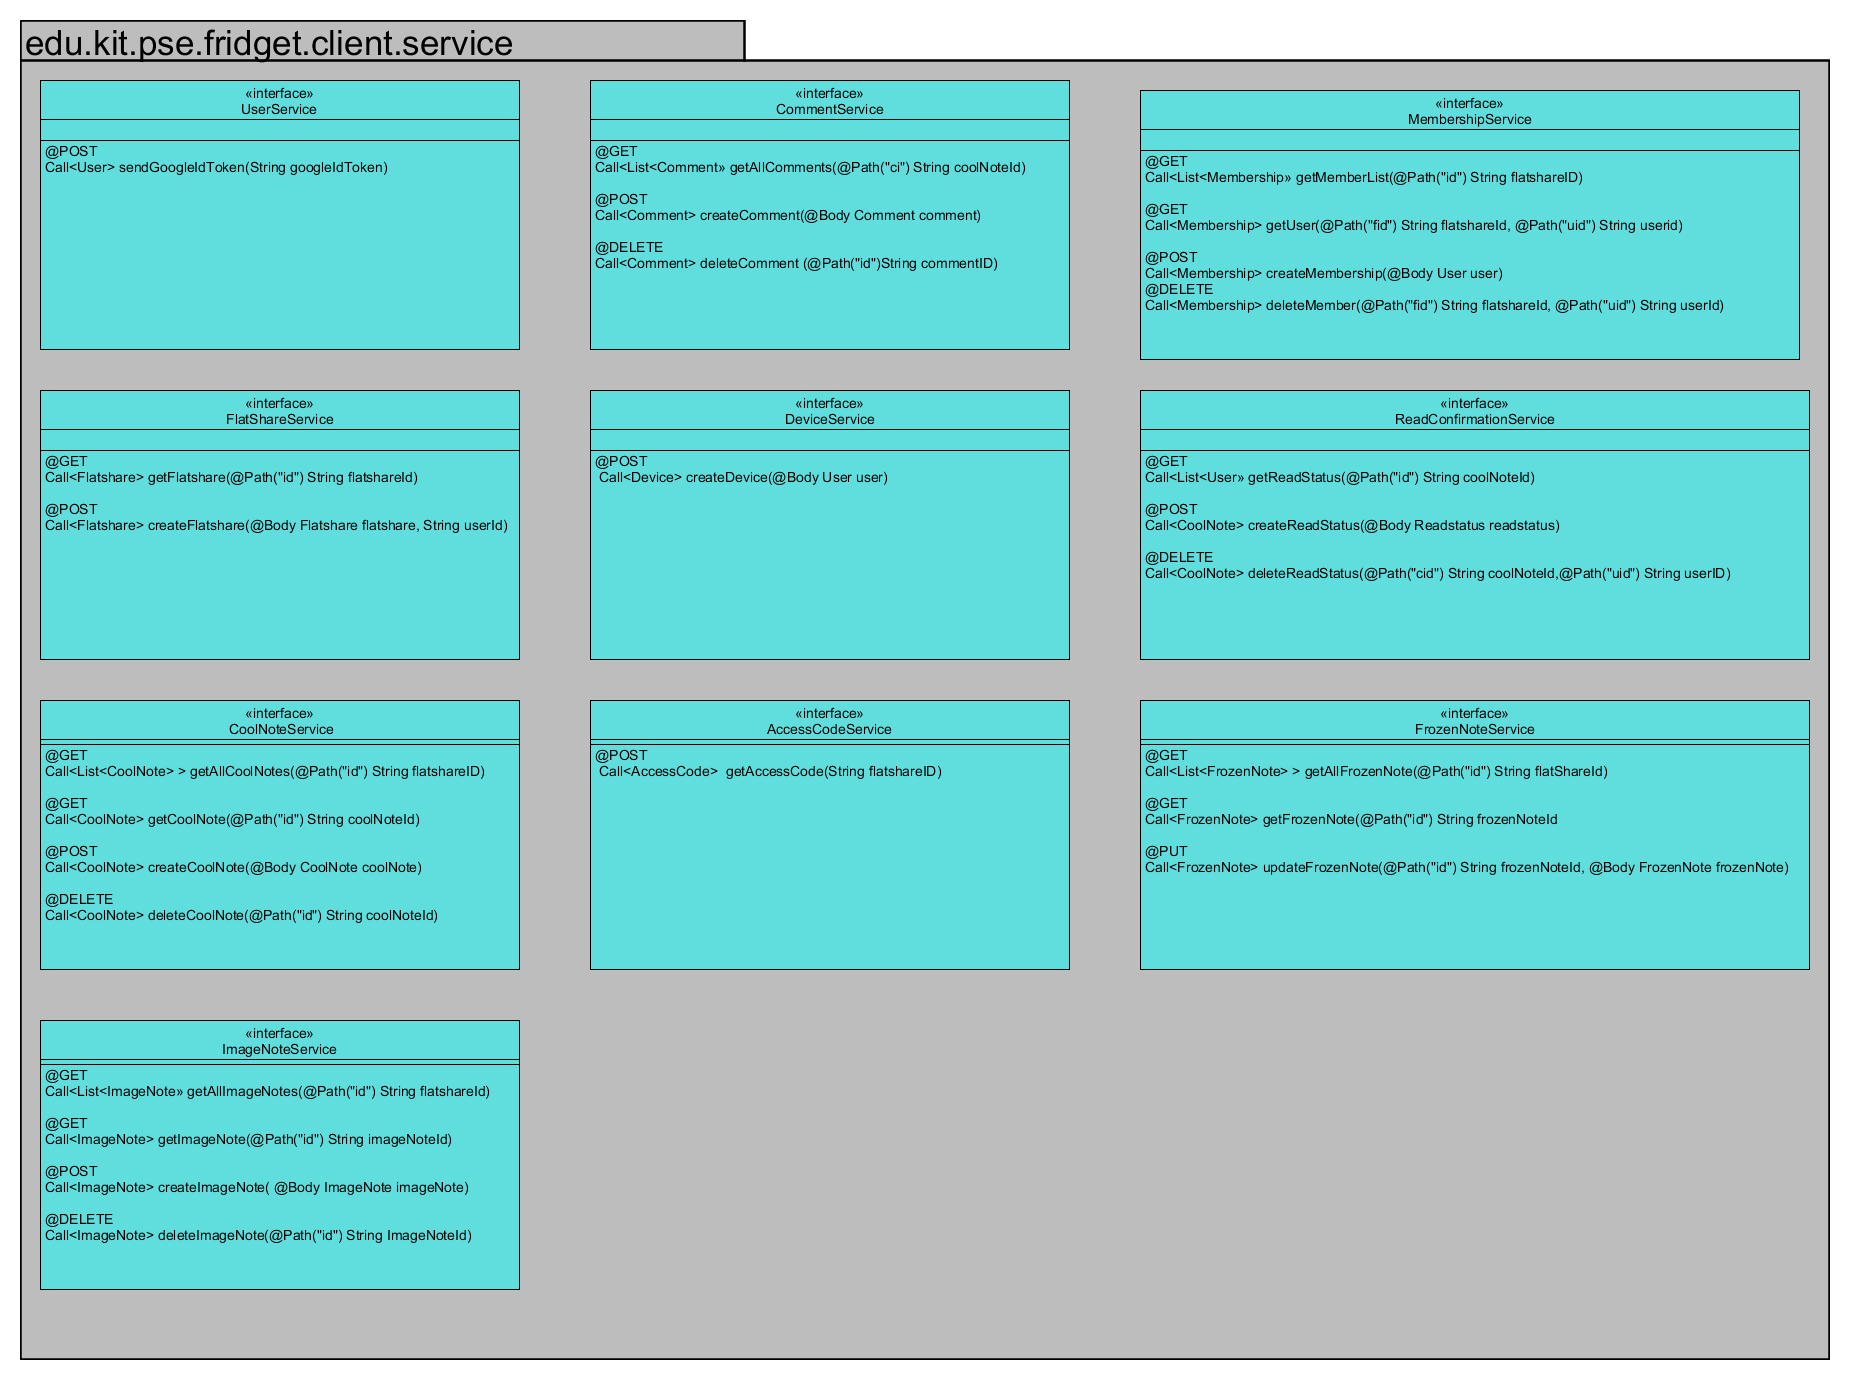
\includegraphics[scale = .26]{service.png}
	       \caption{Klassen des Services}
	      \end{figure}	
	\subsubsection{\texttt{public interface UserService}}
\textit{Dieses Interface dient dazu, dem Nutzer zu ermöglichen sein bestehendes Google Account zum Login zu verwenden. Dabei sendet der Client beim Login ein Token, welches er vom GoogleServer erhält. Dort wird der Token an den GoogleServer gesendet, dadurch erhält der Server die Google Client Id. Diese wird dauerhaft gespeichert.}\\

	\textbf{Methoden} \\
		\begin{itemize}
		\item{@GET\\ Call<User> getGoogleIdToken(String loginData)}

		\textit{Diese Methode ruft den GoogleToken vom Goolge API Server ab}

		\textbf{Parameter} \\
	loginData - Logindaten des Users

		\textbf{Rückgabewert} \\
	GoogleToken

      \item{@POST\\ Call<User> sendGoogleIdToken(String googleIdToken)}

		\textit{Diese Methode sendet den GoogleIdToken an den Server}

		\textbf{Parameter} \\
		googleIdToken - zu sendender GoogleToken

		\textbf{Rückgabewert} \\
	

	 \end{itemize}

	\subsubsection{\texttt{public interface AccesCodeService}}
\textit{Dieses Interface ist für die Synchronisation des Access-Codes mit dem Server zuständig }\\
\\
	\textbf{Methoden} \\
		\begin{itemize}
		\item{@Headers()\\ Call<AccessCode> getAccessCode(String flatShareID)}

		\textit{Diese Methode Diese Methode fordert den Accesscode einer Flatshare an}

		\textbf{Parameter} \\
	flatshareId - übergebende ID der Flatshare

		\textbf{Rückgabewert} \\
	AccessCode der flatshare


	 \end{itemize}

		\subsubsection{\texttt{public interface CommentService }}
\textit{Dieses interfache ist für die Synchronisation der Comments mit dem Server zuständig}\\
\\
	\textbf{Methoden} \\
		\begin{itemize}
		\item{@Headers()\\@GET("comments?cool-note=\{cid\}")\\ Call<List<Comment>> getAllComments(@Path(\grqq cid\grqq)String coolNoteId)}

		\textit{Diese Methode ruft alle Kommentare einer CoolNote ab}

		\textbf{Parameter} \\
	 coolNoteId - die Id der CoolNote 

		\textbf{Rückgabewert} \\
	Alle Comments der zur CoolNoteId zugehörigen CoolNote


      \item{@Headers()\\@POST("/comments")
\\ Call<Comment> createComment(@Body Comment comment)}

		\textit{Diese Methode schickt ein Comment an den Server }

		\textbf{Parameter} \\
		 comment - speichert ein Comment

		\textbf{Rückgabewert} \\
	Ein Comment

	 \item{@Headers()\\@DELETE("/comments/{id}")\\ Call<Comment> deleteComment (@Path(\grqq id\grqq)String commentID)}

		\textit{Diese Methode löscht ein Comment }

		\textbf{Parameter} \\
		 commentID - ID des zu löschenden Comments 



	 \end{itemize}


	\subsubsection{\texttt{public interface CoolNoteService }}
\textit{Dieses Interface ist für die Synchronisation der CoolNotes mit dem Server zuständig}\\
\\
	\textbf{Methoden} \\
		\begin{itemize}
		\item{@Headers()\\@GET("/cool-notes?flatshare={id}")\\ Call<List<CoolNote>> getAllCoolNotes(@Path(\grqq id\grqq) String flatshareID)} 

		\textit{Diese Methode ruft alle CoolNotes einer flatshare ab}

		\textbf{Parameter} \\
	flatshareId - Die flatshare der abzurufenden CoolNotes

		\textbf{Rückgabewert} \\
	Alle Cool Notes

      \item{@Headers() \\ @GET("/cool-notes/{id}")\\ Call<CoolNote> getCoolNote(@Path(\grqq id\grqq) String coolNoteId)}

		\textit{Diese Methode ruft den Inhalt einer CoolNote ab }

		\textbf{Parameter} \\
		coolNoteId - Die Id der CoolNote 

		\textbf{Rückgabewert} \\
	Inhalt der zu der CoolNoteId gehörenden CoolNote

      \item{@Headers() \\ @POST("/cool-notes")\\ Call<CoolNote> createCoolNote(@Body CoolNote coolNote)}

		\textit{Diese Methode schickt eine neue CoolNote an den Server }

		\textbf{Parameter} \\
		coolNoteI - Die CoolNote 

		\textbf{Rückgabewert} \\
	CoolNote


      \item{@Headers() \\ @DELETE("/cool-notes/{id}")\\ Call<CoolNote> deleteCoolNote(@Path(\grqq id\grqq) String coolNoteId)}

		\textit{Diese Methode löscht eine CoolNote }

		\textbf{Parameter} \\
		coolNoteId - Die Id der CoolNote 


	 \end{itemize}


	\subsubsection{\texttt{public interface  FlatShareService }}
\textit{Dieses Interface verwaltet die Synchronisation der Flatshare mit dem Server}\\
\\
	\textbf{Methoden} \\
		\begin{itemize}
		\item{@Headers()\\ @POST ("/flatshares") \\
Call<Flatshare> createFlatshare(@Body Flatshare flatshare, String userId)
}

		\textit{Diese Methode erstellt eine neue Flatshare auf dem Server
}

		\textbf{Parameter} \\
	flatshare - Name der zu erstellenden flatshare
	userID - ID des Users, der die flatshare erstellt

		\textbf{Rückgabewert} \\
	Flatshare

      \item{@Headers()\\  @GET("/flatshares/{id}")\\ Call<Flatshare> getFlatshare(@Path(\grqq id\grqq) 					String flatshareId)}

		\textit{Diese Methode ruft eine Flatshare Daten vom Server ab }

		\textbf{Parameter} \\
		flatshareId - die ID der aufgerufenen Flatshare 

		\textbf{Rückgabewert} \\
	Flatshare


	 \end{itemize}



	\subsubsection{\texttt{public interface FrozenNoteService }}
\textit{Dieses Interface ist für die synchronisation der FrozenNotes mit dem Server zuständig}\\
\\
	\textbf{Methoden} \\
		\begin{itemize}
		\item{@Headers\\ @GET("/frozen-notes?flatshare={id}")\\
Call<List<FrozenNote>> getAllFrozenNote(@Path(\grqq id\grqq) String flatShareId)}

		\textit{Diese Methode ruft die FrozenNotes vom Server ab}

		\textbf{Parameter} \\
	flatshareId -  die ID der aufgerufenen Flatshare  

		\textbf{Rückgabewert} \\
	FrozenNote

      \item{@Headers\\ @GET("/frozen-notes/{id}")\\ Call<FrozenNote> getFrozenNote(@Path(\grqq id\grqq) String frozenNoteId)}

		\textit{Diese Methode ruft den Inhalt einer FrozenNote ab }

		\textbf{Parameter} \\
		frozenNoteId - die ID der aufgerufenen FrozenNote  

		\textbf{Rückgabewert} \\
	FrozenNote

	 \item{@Headers\\ @PUT("/frozen-notes/{id}")\\ Call<FrozenNote> updateFrozenNote(@Path(\grqq id\grqq) String frozenNoteId, @Body FrozenNote frozenNote)}

		\textit{Diese Methode speichert Änderungen  in einer FrozenNote}

		\textbf{Parameter} \\
		frozenNoteId - die ID der aufgerufenen FrozenNote  
		frozenNote - die geänderte FrozenNote
		\textbf{Rückgabewert} \\
	FrozenNote

	 \end{itemize}


	\subsubsection{\texttt{public interface ImageNoteService }}
\textit{Dieses Interface dient zur Synchronisation der ImageCoolNotes mit dem Server}\\
\\
	\textbf{Methoden} \\
		\begin{itemize}
		\item{@Headers()\\ @GET("/image-notes?flatshare={id}")\\
Call<List<ImageNote>> getAllImageNotes(@Path(\grqq id\grqq) String flatshareId)}

		\textit{Diese Methode ruft die ImageCoolNotes vom server ab}

		\textbf{Parameter} \\
	flatshareId - die ID der aufgerufenen Flatshare   

		\textbf{Rückgabewert} \\
	ImageCoolNote

      \item{@Heders\\ @GET("/image-notes/{id}")\\ Call<ImageNote> getImageNote(@Path("\grqq id\grqq") String imageNoteId)}

		\textit{Diese Methode ruft eine ImageNote ab }

		\textbf{Parameter} \\
		 imageNoteId - die ID der aufgerufenen ImageNote  

		\textbf{Rückgabewert} \\
	ImageNote

	\item{@Headers\\ @POST("/image-notes")\\ Call<ImageNote> createImageNote( @Body ImageNote imageNote)}

		\textit{Diese Methode schickt ein ImageNote an den Server}

		\textbf{Parameter} \\
		 imageNote - eine ImageNote  

		\textbf{Rückgabewert} \\
	ImageNote

	     \item{@Headers\\ @DELETE("/image-notes/{id}")\\Call<ImageNote> deleteImageNote(@Path("\grqq id\grqq") String ImageNoteId)}

		\textit{Diese Methode löscht eine ImageNote}

		\textbf{Parameter} \\
		 imageNoteId - Die ID der zu löschenden ImageNote  

	 \end{itemize}


	\subsubsection{\texttt{public interface  MembershipService }}
\textit{Dieses Interface verwaltet die Synchronisation der Members mit dem Server}\\
\\
	\textbf{Methoden} \\
		\begin{itemize}
		\item{@Headers()\\ @GET("/memberships/users?flatshare={id}") \\ Call<List<Membership>> getMemberList(@Path("id") String flatshareID)}

		\textit{Diese Methode ruft die Mitglieder einer Flatshare ab}

		\textbf{Parameter} \\
	flatshareId - die ID der aufgerufenen Flatshare  

		\textbf{Rückgabewert} \\
	MemberList

      \item{@Headers()\\ @GET("memberships?flatshare={fid}\&user ={uid}")\\Call<Membership> getUser(@Path("fid") String flatshareId, @Path(\grqq uid\grqq) String userid)}

		\textit{Diese Methode ruft die Daten eines Members ab}        	
		\textbf{Parameter} \\
		flatshareId - die ID der aufgerufenen Flatshare 
	userId - die ID des aufgerufenen Users

		\textbf{Rückgabewert} \\
      Daten eines Members


      \item{@Headers()\\ @POST("/memberships")\\ Call<Membership> createMembership(@Body User user)}

		\textit{Diese Methode fügt ein neues Member in eine flatshare ein}        	
		\textbf{Parameter} \\
		user - Der User der zu der flatshare hinzugefügt wird 

	      \item{@Headers()\\ @DELETE("/memberships?flatshare={fid}\&user={uid}")\\Call<Membership> deleteMember(@Path("fid") String flatshareId, @Path("uid") String userId)}

		\textit{Diese Methode löscht ein Member}        	
		\textbf{Parameter} \\
		flatshareId - die ID der aufgerufenen Flatshare 
	userId - die ID des aufgerufenen Users


	 \end{itemize}

	\subsubsection{\texttt{public interface  ReadConfirmationService }}
\textit{ Dieses Interface synchronisasiert den gelesen Status mit dem Server}\\
\\
	\textbf{Methoden} \\

    \begin{itemize}
		\item{@Headers()\\@GET("/read-confirmations/users?cool-note={id}") \\ Call<List<User>> getReadStatus(@Path(\grqq id\grqq) String coolNoteId)}

		\textit{Diese Methode ruft den gelesen Status vom Server ab}

		\textbf{Parameter} \\
	 coolNoteId - Die ID der betreffenden CoolNote

		\textbf{Rückgabewert} \\
	ReadStatus

	\item{@Headers()\\ @POST("/read-confirmations") \\ Call<CoolNote> createReadStatus(@Body Readstatus readstatus) } \todo{Mins Klasse übernehmen}

		\textit{Diese Methode setzt die Checkbox auf markiert}

		\textbf{Parameter} \\
	 readstatus - zeigt den gelesen Status einer CoolNote an

		\textbf{Rückgabewert} \\
	ReadStatus



	\item{@Headers()\\ @DELETE("/read-confirmations?cool-note={cid}\&user={uid}")}
\\Call<CoolNote> deleteReadStatus(@Path("cid") String coolNoteId,
			     @Path(\grqq uid\grqq) String userID);

		\textit{Diese Methode setzt die Checkbox auf unmarkiert}

		\textbf{Parameter} \\
	coolNoteID - die ID der aufgerufenen CoolNote
	userID - die ID des aufgerufenen Users

	
	 \end{itemize}


	\subsubsection{\texttt{public interface DeviceService }}
\textit{Dieses Interface synchronisiert die Device-Daten mit dem Server}\\
\\
	\textbf{Methoden} \\
		\begin{itemize}
		\item{@Headers()\\@POST("/devices") \\ Call<Device> createDevice(@Body User user)}

		\textit{Diese Methode fügt ein Device zu einer flatshare hinzu}

		\textbf{Parameter} \\
	 user - der zu dem Device zugehörige User 

		\textbf{Rückgabewert} \\


	 \end{itemize}




